\subsection{Astrobiology}
\label{sec:Astrobiology-Background}

Extremophiles thrive in physically and/or chemically extreme conditions, which are detrimental to most of life on Earth as we know it. These organisms and microbes have been found everywhere, from deep underwater volcano vents to buried ice lakes in Antarctica \cite{Extremophiles}.  As shown in Table~\ref{tab:astrobiotable}, fungi and bacterial spores have previously been found in the stratosphere. Arguably, each successful collection expedition of at least \SI{30}{\kilo\meter} into the upper atmosphere provides information that could be useful in determining what life forms can exist inside and outside of Earth's biosphere. Today, the most common altitude for bacterial collection in the atmosphere occurs in the range of approximately \SIrange{10}{20}{\kilo\meter} above Earth's surface; very little data exists on microbiological samples captured in the stratosphere. Conditions at altitudes of \SIrange{30}{40}{\kilo\meter} are extreme in temperature, pressure and radiation. 

	
%\begin{figure}[H]
%\centering
%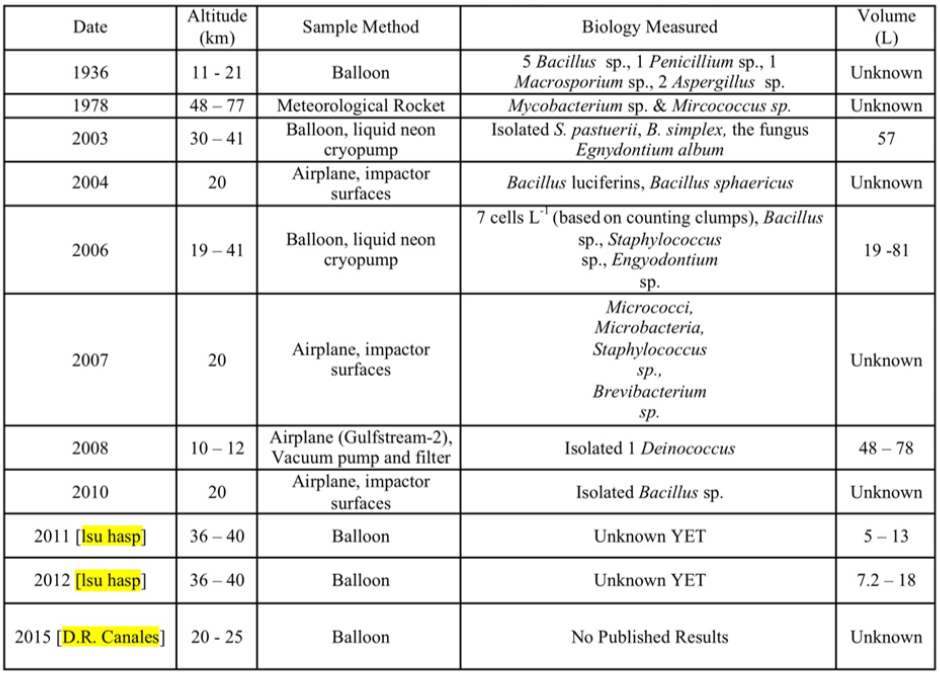
\includegraphics[width=1\textwidth]{./Figures/AstroChart.PNG}
%\caption{}
%\label{fig:AstroHist}
%\end{figure} 




Our experiment is an attempt to further develop our technique for capturing microorganisms in the upper atmosphere, as demonstrated during our 2017~\cite{SORA} flight.  We took inspiration from the LSU HASP 2011, 2012, 2013 flights~\cite{LSU} and from research by D.R. Canales~\cite{canales}.  This flight will also help us further understand our findings from our first flight, and to maybe fully culture these rare microorganisms. We will use two of the KNF N84-4 commercial gas-sampling diaphragm vacuum pumps to sample the air at approximately \SI{33}{\kilo\meter} above Earth's surface. The samples we hope to collect are an important part to expanding our understanding of Earth's biosphere and further studies could provide more insight on how life can be distributed on Earth, and ultimately, through outer-space.

\begin{table}[!ht]
\centering
\caption{History of Microbiological Sampling of the stratosphere~\cite{SORA}.} 
\label{tab:AstroHist} 
\bigskip
\begin{tabular}{|c|c|c|p{6cm}|c|}
\hline
\multicolumn{1}{|c|}{\bfseries Date} & \minitab{c}{\bf Altitude}{\bf (km)} &  \multicolumn{1}{c|}{\bfseries Sample Method} & \multicolumn{1}{p{6cm}|}{\bfseries Biology Measured} & \multicolumn{1}{c|}{\bfseries Volume} \\
\hline
    1936	& 11 - 12 	& Balloon			 			& \minitab{l}{5 Bacillus sp., 1 Penicillium sp.,}{1 Macrosporium sp., 2 Aspergillus sp.} 			& $Unknown$ \\ \hline
    1978	& 48 - 77 	&Meteorological Rocket	 		& Mycobacterium sp., Mircococcus sp.					       							& $Unknown$ 	\\ \hline
    2003	& 30 - 41	& Balloon, liquid neon cryopump	& \minitab{l}{Isolated S. pastuerii, B. simplex,}{the fungus, Egnydontium album}       				& $57$	\\ \hline    
    2004	& 20	 	&Airplane, Impactor Surfaces 	 	& Bacillus luciferins, Bacillus sphaericus			       									& $Unknown$ 	\\ \hline
    2006	& 19 - 41	& Balloon, Liquid Neon Cryopump 	& \minitab{l}{7 cells L-1 (counting clumps), Bacillus sp.,}{Staphylococcus sp., Engyodontium sp.}	& $19-81$ \\ \hline
    2007	& 20	       	& Airplane, Impactor Surfaces 		& \minitab{l}{Micrococci, Microbacteria,}{Staphylococcus sp., Brevibacterium sp.}    				& $Unknown$ \\ \hline
    2010	& 20	       	& Airplane, Impactor Surfaces 		& Isolated Bacillus sp.							     								& $Unknown$\\ \hline
    2017	& 32	       	& Balloon, liquid medium and vacuum pump	&  Mulitple findings~\cite{SORA}							     								& $Unknown$\\ \hline
\end{tabular}
\label{tab:astrobiotable}
\medskip
\end{table}
